\documentclass[tikz,border=8pt]{standalone}
\usetikzlibrary{arrows.meta}
\begin{document}
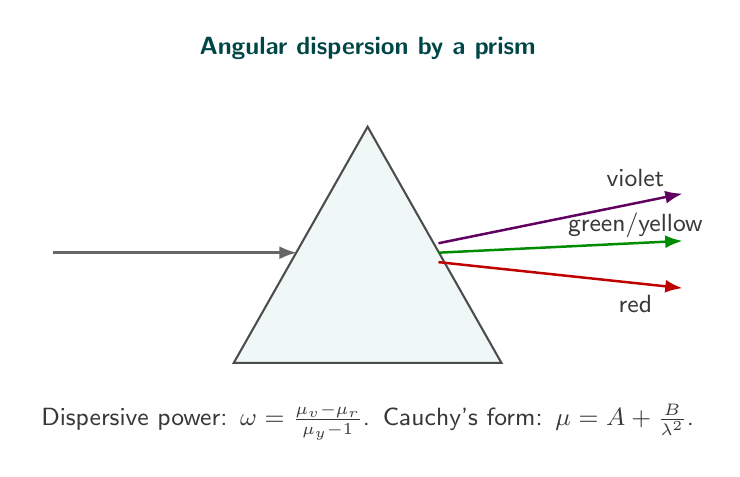
\begin{tikzpicture}[
  ray/.style={-{Latex[length=2.2mm]},line width=0.9pt},
  line/.style={draw=black!70,line width=0.75pt},
  label/.style={font=\sffamily\small,text=black!78},
  title/.style={font=\sffamily\bfseries\small,text=teal!55!black},
]
\node[title] at (0,3.0) {Angular dispersion by a prism};
\draw[line,fill=teal!6] (0,2)--(-1.7,-1)--(1.7,-1)--cycle;
\draw[ray,draw=black!60] (-4,0.4)--(-0.9,0.4);
\draw[ray,draw=violet!75!black] (0.9,0.52)--(4,1.15);
\draw[ray,draw=green!55!black] (0.9,0.40)--(4,0.55);
\draw[ray,draw=red!75!black] (0.9,0.28)--(4,-0.05);
\node[label] at (3.4,1.35) {violet};
\node[label] at (3.4,0.75) {green/yellow};
\node[label] at (3.4,-0.25) {red};
\node[label,align=center,text width=8.4cm] at (0,-1.75)
  {Dispersive power: $\omega=\frac{\mu_v-\mu_r}{\mu_y-1}$. Cauchy's form: $\mu=A+\frac{B}{\lambda^2}$.};
\end{tikzpicture}
\end{document}
